\section{Resolución Problema 1} 
Para dar solución a este problema se utiliza  el método de las 6’D, que está compuesto de seis etapas, cada una de las cuales consta de una serie de pasos, descripción del
problema, definición de solución, diseño de la solución,
desarrollo de la solución, depuración y pruebas y
documentación. \\



Este programa en Java resuelve dos problemas de geometría analítica. Primero, determina la ecuación de una recta que pasa por los puntos A y B usando el método:
\[
\text{ $y = mx + b$ }
\]
 Luego, calcula el ángulo interno entre la recta y el eje horizontal utilizando el método de la tangente inversa  $"a "$ = arctan(m)".
\subsection{\textbf{Descripcion del problema:}}
\begin{itemize}

    \item Dados 2 puntos A y B con coordenadas x1, y1 y x2, y2 respectivamente. Regresar la ecuación de la recta y el ángulo interno α que se forma entre el eje horizontal y la recta.
    \end{itemize}
\subsection{\textbf{Diseño de la solución:}}
La solución implica calcular la pendiente de la recta que pasa por los puntos A y B y utilizarla para obtener la ecuación de la recta en la forma y = mx + b, donde m es la pendiente y b es la intersección en el eje y. Una vez obtenida la ecuación de la recta, se puede calcular el ángulo interno utilizando la función trigonométrica arcotangente.
\begin{figure}[h!]
    \centering
    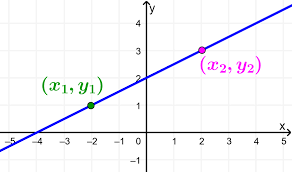
\includegraphics[width = 6.5 cm]{LaTeX/latex-imagenes/grafica-rectapendiente.png}
    \caption{Gráfica de dos puntos en la recta.}
    \label{fig:GraficaEcuacionRecta}
\end{figure} 
\subsection{\textbf{\textit{Diseño de solución }}}
\begin{itemize}
  \item Calcular la pendiente (m) de la recta utilizando la fórmula:
\begin{equation}
    m = (y2 - y1) / (x2 - x1)
\end{equation}
   
  \item  Calcular el término independiente (b)  utilizando la fórmula 
 \begin{equation}
     b = y1 - mx1.
\end{equation}
  \item Obtener la ecuación de la recta
   \begin{equation}
     y = mx + b.
\end{equation}
  \item Calcular el ángulo interno (a) utilizando la fórmula
    \begin{equation}
      a = tan^(-1)(m)
    \end{equation}
\end{itemize}
Utilizando este método, puedes encontrar la ecuación de la recta a partir de dos puntos. Recuerda que si los dos puntos son idénticos la recta será una linea vertical
\cite{rectaPendiente}

\subsection{ \textbf{\textit{Diagrama de flujo }}}

\begin{figure}[H]
    \centering
    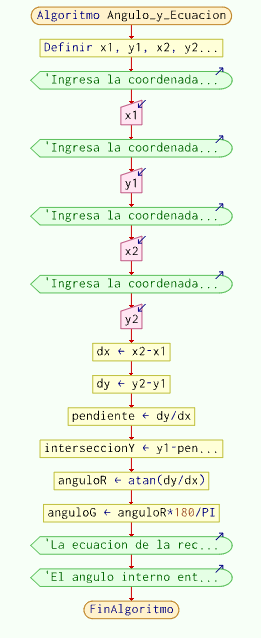
\includegraphics[width=6cm]{LaTeX/latex-imagenes/Diagrama de flujo.png}
    \caption{Diagrama de flujo usado para la solución del problema}
\end{figure}
\subsection{\textbf{Desarrollo de la solución:}}
// Comienza solicitando al usuario dos puntos $A(x_{1}, y_{1})$ y $B(x_{2}, y_{2})$.

\begin{lstlisting}[style=javaStyle]
    Scanner sc = new Scanner(System.in);
    // Solicita datos del primer punto
    System.out.println("Ingresa la coordenada x1: ");
    double x1 = sc.nextDouble();
    System.out.println("Ingresa la coordenada y1: ");
    double y1 = sc.nextDouble();
        
    // Solicita datos del segundo punto
    System.out.println("Ingresa la coordenada x2: ");
    double x2 = sc.nextDouble();
    System.out.println("Ingresa la coordenada y2: ");
    double y2 = sc.nextDouble();
\end{lstlisting}
//Se  calcula la diferencia entre coordenadas, con el fin de determinar la distancia o el desplazamiento entre dos puntos en un sistema de coordenadas.
\begin{lstlisting}[style=javaStyle]
    // Calcula la diferencia entre coordenadas
    double dx = x2 - x1;
    double dy = y2 - y1;
        
\end{lstlisting}
//Calculamos la pendiente usando la  formula 
 $m = (y2-y1) / (x2-x1)$
Una vez obtenida la pendiente, obtenemos la intersección con el eje "Y"
\begin{lstlisting}[style=javaStyle]
        // Calcula la pendiente y la intersección con el eje Y
        double pendiente = dy / dx;
        double interseccionY = y1 - pendiente * x1;
        
\end{lstlisting}
    // Calcula el ángulo en radianes
        
\begin{lstlisting}[style=javaStyle]
     double anguloR = Math.atan2(dy, dx);
\end{lstlisting}
    // Convierte el ánguloR a grados
\begin{lstlisting}[style=javaStyle]
    double anguloG = Math.toDegrees(anguloR);
\end{lstlisting}
    //Finalmente obtenemos como resultado la ecuación de la recta que pasa a través de dos puntos dados, A y B. 
    Además del el ángulo interno formado entre el eje horizontal y la recta.
\begin{lstlisting}[style=javaStyle]
    
        // Imprime la ecuación y el ángulo interno
        System.out.println("La ecuación de la recta es: y = " + pendiente + "x + " + interseccionY);
        System.out.println("El ángulo interno entre la recta y el eje horizontal es: " + anguloG + " grados");

\end{lstlisting}

\subsection{\textbf{\textit{Código general}}}
\begin{lstlisting}[style=javaStyle]
package com.mycompany.proyecto;
import java.util.Scanner;
/**
 *
 * @author Frey
 */
public class Angulo_y_Ecuacion {
    public static void main(String[] args) {
        Scanner sc = new Scanner(System.in);
        // Solicita datos del primer punto
        System.out.println("Ingresa la coordenada x1: ");
        double x1 = sc.nextDouble();
        System.out.println("Ingresa la coordenada y1: ");
        double y1 = sc.nextDouble();
        
        // Solicita datos del segundo punto
        System.out.println("Ingresa la coordenada x2: ");
        double x2 = sc.nextDouble();
        System.out.println("Ingresa la coordenada y2: ");
        double y2 = sc.nextDouble();
        
        // Calcula la diferencia entre coordenadas
        double dx = x2 - x1;
        double dy = y2 - y1;
        
        // Calcula la pendiente y la intersección con el eje y
        double pendiente = dy / dx;
        double interseccionY = y1 - pendiente * x1;
        
        // Calcula el ángulo en radianes
        double anguloR = Math.atan2(dy, dx);
        
        // Convierte el ánguloR a grados
        double anguloG = Math.toDegrees(anguloR);
        
        // Imprime la ecuación y el ángulo interno
        System.out.println("La ecuación de la recta es: y = " + pendiente + "x + " + interseccionY);
        System.out.println("El ángulo interno entre la recta y el eje horizontal es: " + anguloG + " grados");
    }
}
\end{lstlisting}


\subsection{\textbf{Depuración y pruebas:}}
\begin{figure}[H]
    \centering
    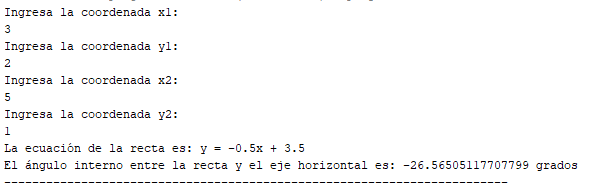
\includegraphics[width=8cm]{LaTeX/latex-imagenes/prueba de escritorio2.png}
    \caption{Prueba de escritorio.}
\end{figure}
\begin{figure}[H]
    \centering
    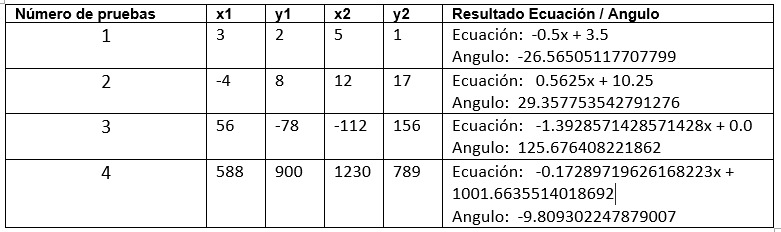
\includegraphics[width=10cm]{LaTeX/latex-imagenes/TABLA.jpg}
    \caption{Tabla de corridas.}
\end{figure}
